%%%%%%%% ICML 2018 EXAMPLE LATEX SUBMISSION FILE %%%%%%%%%%%%%%%%%

\documentclass{article}

% Recommended, but optional, packages for figures and better typesetting:
\usepackage{microtype}
\usepackage{graphicx}
\usepackage{subfigure}
\usepackage{booktabs} % for professional tables

% hyperref makes hyperlinks in the resulting PDF.
% If your build breaks (sometimes temporarily if a hyperlink spans a page)
% please comment out the following usepackage line and replace
% \usepackage{icml2018} with \usepackage[nohyperref]{icml2018} above.
\usepackage{hyperref}

% Attempt to make hyperref and algorithmic work together better:
\newcommand{\theHalgorithm}{\arabic{algorithm}}

% Use the following line for the initial blind version submitted for review:
%\usepackage{icml2018}

% If accepted, instead use the following line for the camera-ready submission:
\usepackage[accepted]{icml2018}

% other packages
\usepackage{verbatim}
\usepackage{url}
\usepackage{amsmath,amssymb}

\graphicspath{ {images/} }

% The \icmltitle you define below is probably too long as a header.
% Therefore, a short form for the running title is supplied here:
\icmltitlerunning{Generalized Multi-Agent Reinforcement Learning}

\begin{document}

\twocolumn[
\icmltitle{Generalized Multi-Agent Reinforcement Learning in \\ 
	       Cooperative and Competitive Environments}

% It is OKAY to include author information, even for blind
% submissions: the style file will automatically remove it for you
% unless you've provided the [accepted] option to the icml2018
% package.

% List of affiliations: The first argument should be a (short)
% identifier you will use later to specify author affiliations
% Academic affiliations should list Department, University, City, Region, Country
% Industry affiliations should list Company, City, Region, Country

% You can specify symbols, otherwise they are numbered in order.
% Ideally, you should not use this facility. Affiliations will be numbered
% in order of appearance and this is the preferred way.
\icmlsetsymbol{equal}{*}

\begin{icmlauthorlist}
\icmlauthor{Diana Huang}{equal}
\icmlauthor{Shalini Keshavamurthy}{equal}
\icmlauthor{Nitin Viswanathan}{equal}
\end{icmlauthorlist}


% You may provide any keywords that you
% find helpful for describing your paper; these are used to populate
% the "keywords" metadata in the PDF but will not be shown in the document
\icmlkeywords{Machine Learning, ICML}

\vskip 0.3in
]

% this must go after the closing bracket ] following \twocolumn[ ...

% This command actually creates the footnote in the first column
% listing the affiliations and the copyright notice.
% The command takes one argument, which is text to display at the start of the footnote.
% The \icmlEqualContribution command is standard text for equal contribution.
% Remove it (just {}) if you do not need this facility.

%\printAffiliationsAndNotice{}  % leave blank if no need to mention equal contribution
%\printAffiliationsAndNotice{\icmlEqualContribution} % otherwise use the standard text.

\begin{comment}
\begin{abstract}
This document provides the current progress on our project. The objective of the 
\end{abstract}
\end{comment}

\section{Introduction}
\label{submission}

There are many applications where multiple agents need to learn how to act together, such as multiplayer games ~\cite{multigames}, multi-robot control ~\cite{multirobot}, communication scenarios ~\cite{communication}, and even self-play ~\cite{selfplay}.

Traditional reinforcement learning approaches focus on training a single agent and as a result, they do not work well on multi-agent problems because the environment for any single agent changes over time as other agents change their policies, leading to instability during training and high variance in results ~\cite{unstable}. Additionally, experience replay as used with Q-learning cannot be applied in multi-agent scenarios, significantly hampering stable learning.

In addition to applying traditional approaches, prior work on multi-agent reinforcement learning (MARL) has attempted to develop new approaches specifically for multi-agent scenarios. In particular, recent work has achieved significantly improved results by modifying existing RL algorithms to train agents while incorporating information from the other agents, creating multi-agent deep deterministic policy gradients (MADDPG) \cite{maddpg}. However, one key limitation of MADDPG and other related approaches is that they do not generalize well to larger numbers of agents due to the growing computational complexity of incorporating information from all agents in training. Given the extensive training time necessary for even smaller scenarios, it is not feasible to retrain new networks for different possible numbers of agents.

We plan to develop a generalized training approach for multi-agent scenarios to find policies that scale well when applied in environments with varying numbers of agents. We do so by modifying the training process of MADDPG to train agents using only information from nearby agents instead of information from every agent, allowing agents to learn to make decisions based off of the location of a fixed number of nearby agents. As a baseline, we have implemented a REINFORCE policy gradient approach and will also re-implement MADDPG. We will compare these algorithms against our generalized algorithm to see how they perform in scenarios with various numbers of agents.

\section{Approach}

\subsection{Environment}

We use an OpenAI Gym environment with a variety of multi-agent cooperative and competitive scenarios as well as environments that allow communication between agents ~\cite{openaigym}. For our initial explorations, we focused on the cooperative navigation environment where there are N agents that can move in a 2-D world and N fixed landmarks. All agents are rewarded based on the collective distance between agents and landmarks, and punished for colliding with each other. In order to maximize reward, each agent needs to learn to move to a different landmark while avoiding collisions with other agents.

\begin{figure}
\begin{center}
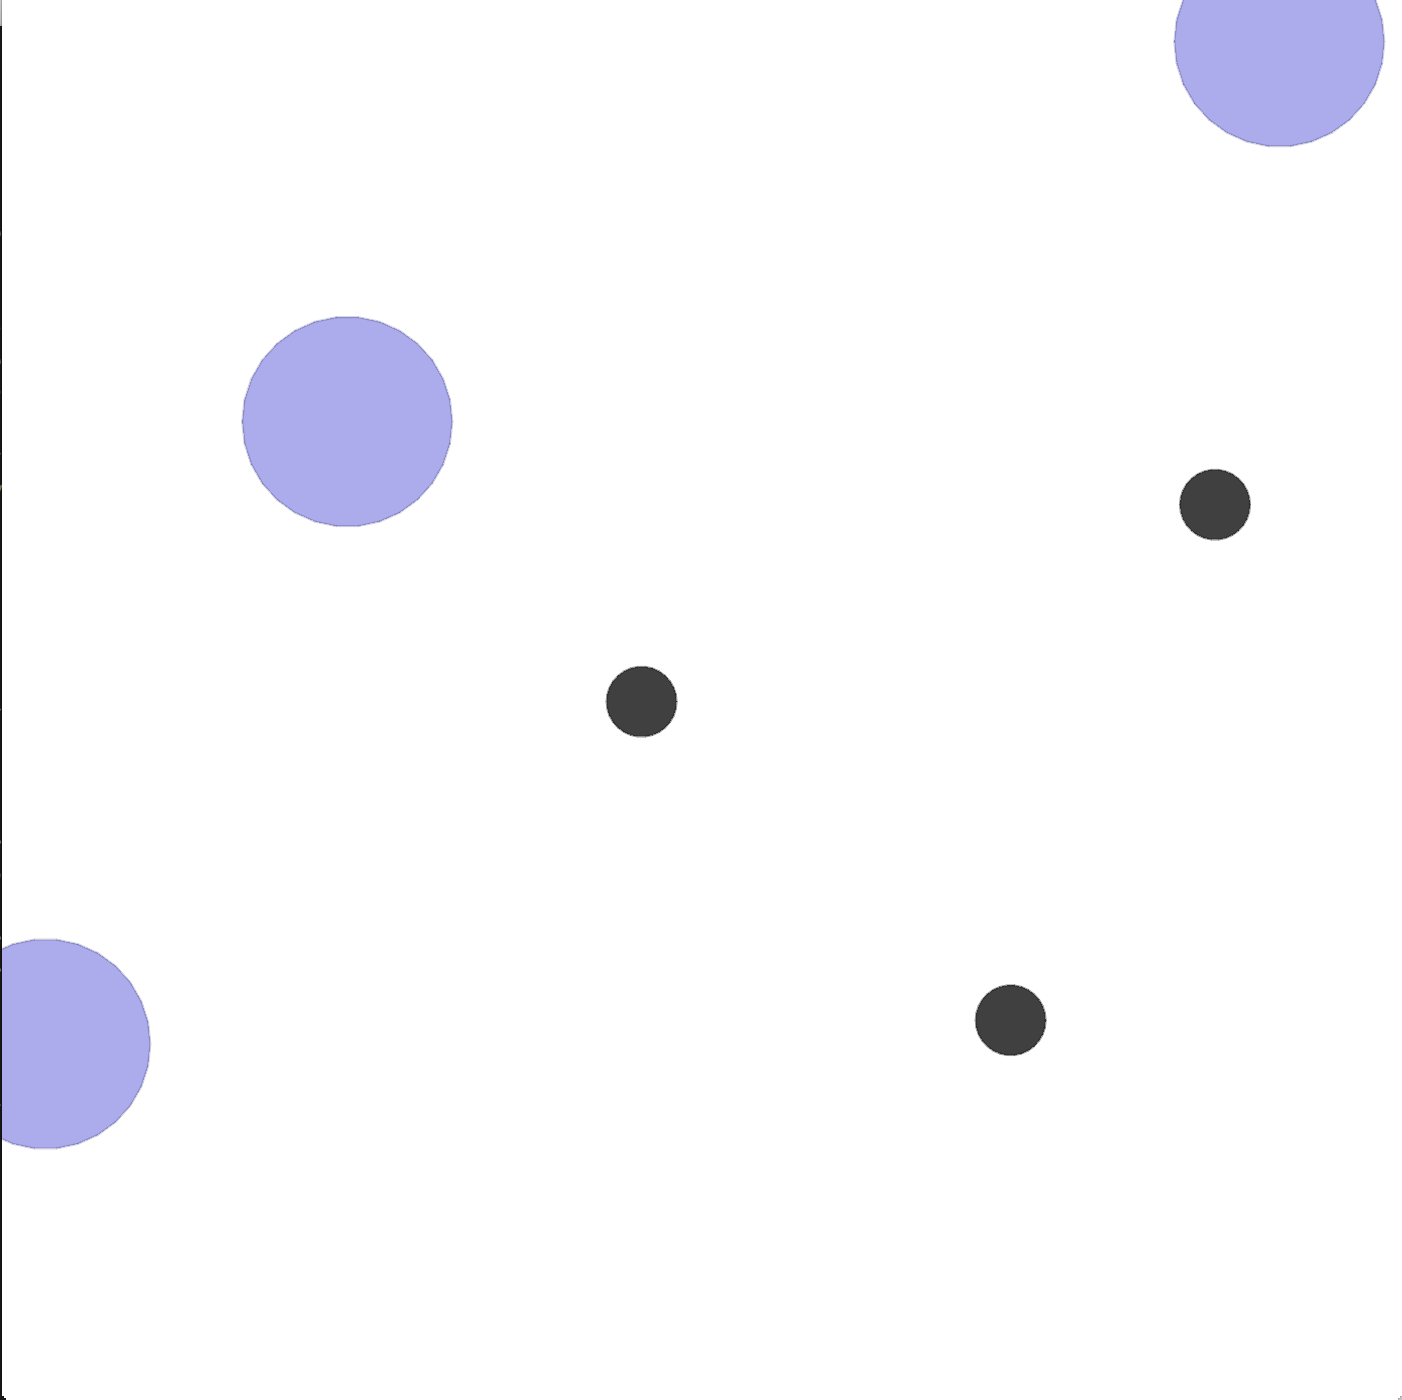
\includegraphics[scale=0.15]{env-image}
\end{center}
\caption{Example environment initialization. Blue circles are agents and black dots are target landmarks.}
\end{figure}

The observation space for the cooperative navigation environment consists of information about every agent's position and velocity, relative distance to all of the landmarks, and relative distance to every other agent. An agent acts by choosing to move either up, down, left, right, or taking a no-move action. During test time, an agent can only take actions based on it's own observations of the world, but during train time, MADDPG and other approaches tailored to multi-agent scenarios will allow agents to use observations from other agents as well.

\subsection{Methods}
As an initial baseline, we have implemented the REINFORCE algorithm for multi-agent scenarios. With REINFORCE, every agent trains its own independent policy network based on its observation of the environment and the possible actions it can take. Even after applying a baseline and advantage normalization we did not expect REINFORCE to perform well due to the potential for very large variance in the gradient. From a single agent's perspective not only does the world change as other agents move, but the policies other agents follow change as well. Additionally, individual agents might not always get the correct gradient signal as an agent could take a good action but if other agents took bad actions, leading to overall decrease in reward, the gradient for the agent taking the correct action could still be negative. Nevertheless, REINFORCE serves as a baseline for comparing against more sophisticated approaches.

We are currently in the process of re-creating MADDPG from ~\cite{maddpg} as a second baseline. MADDPG takes DDPG and tailors it to multi-agent scenarios, resulting in significantly better performance than single-agent methods such as REINFORCE and DDPG. MADDPG trains separate policy networks for every agent, but uses a centralized action-value function that incorporates information across all agents to ensure a more stable learning process. 

Consider a game with $N$ agents, and let $\pi = \{\pi_1, ..., \pi_N\}$ be the associated set of agent policies that are parametrized by $\theta_1, ..., \theta_N$. The gradient update for MADDPG for agent $i$, $\nabla_{\theta_i} J(\theta_i)$, is:

$$\nabla_{\theta_i}J(\theta_i) = \mathbb{E}_{s, a_i}[\nabla_{\theta_i}log \pi_i(a_i|o_i)Q^{\pi}_i(x, a_1, ..., a_N)]$$

Where $o_i$ is the local observation of the environment by agent $i$, $x$ is the full state information across all agents, and $Q^{\pi}_i$ is a centralized action-value function that takes as input the actions of all agents. By incorporating the actions of all agents into the action-value function, instead of only each individual agent, MADDPG produces better and more stable results than traditional policy gradient or Q-learning approaches.

After re-implementing MADDPG, we plan to modify the original MADDPG algorithm to train agents in a generalized way. More specifically, we will still maintain a centralized critic function for each agent, but instead of taking actions from all agents as input, only actions from neighboring agents would be considered. This is to make the number of parameters in the Q network constant, rather than linear to number of agents in the environment. Thus, the computational complexity for updating the Q network is also capped.

\subsection{Experiments}

For the milestone, we have been focusing on the cooperative navigation environment as mentioned previously. Our primary evaluation metric has been average reward, which in this environment corresponds to the distance between agents and the target landmarks while also accounting for collisions that occur along the way. In addition to average reward, in the future we will also look at success rate, where we define success as agents successfully reaching the target landmarks with 0 collisions, no matter how long it took for this to occur. This way, we will evaluate the policy that our algorithm converges to not only based on how quickly it leads agents to reach the landmarks, but how often it leads agents to the landmarks.

We will evaluate our model performance during both train and test time. During train time, we will see how quickly we are able to reach convergence and how stable the training process is across the different implemented methods. During test time, we will compare our different methods with the average reward over many trials as well as the variance, and also see how performance changes as we change the number of agents present to test generalization. The original authors of MADDPG only tested scenarios with a maximum of 3 agents , so we will try increasing this to 4 to 6 agents and seeing how performance changes.

For our re-created version of MADDPG, we expect to match results from the original MADDPG paper as closely as possible when evaluating on up to 3 agents. For more than 3 agents, we will compare results from our re-created MADDPG and the modified, generalized version of MADDPG. We aim to have the modified MADDPG perform at least as well as the re-created MADDPG but train faster than the re-created MADDPG.




\subsection{Results}

\begin{figure}
\centering
    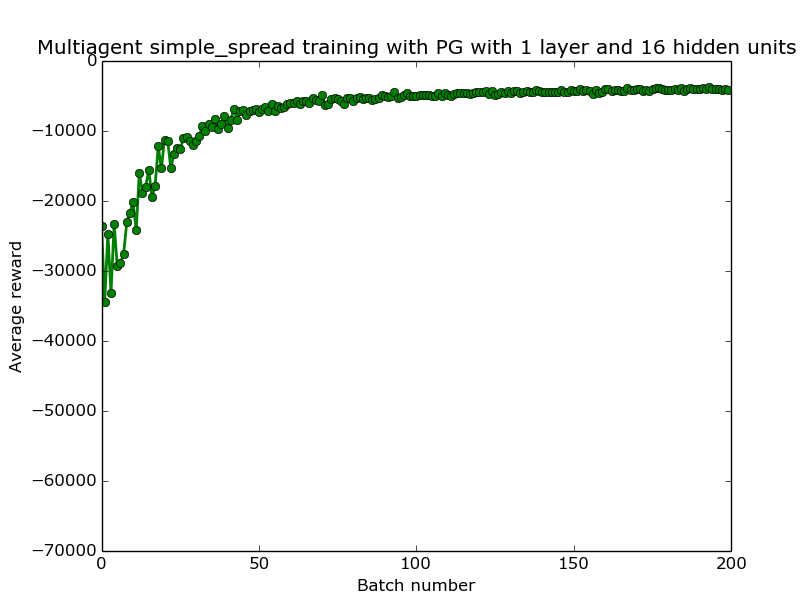
\includegraphics[scale=0.25]{pg_1_16_gamma1}
    \caption{Average reward over time when training PG with 1 layer and 16 hidden units.}
\label{fig:pg_1_16_gamma1}
\end{figure}

\begin{figure}
\centering
    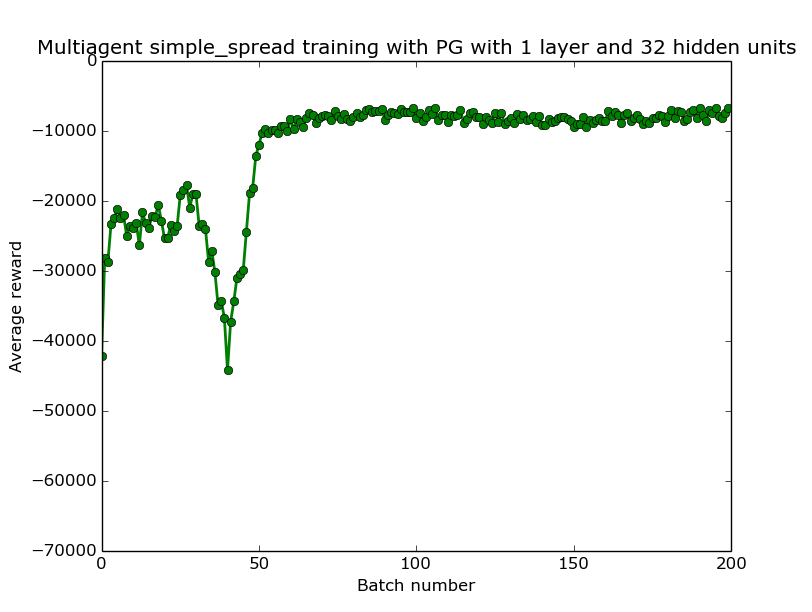
\includegraphics[scale=0.25]{pg_1_32_gamma95}
    \caption{Average reward over time when training PG with 1 layer and 32 hidden units, gamma=0.95, learning rate=2e-3.}
\label{fig:pg_1_32_gamma95}
\end{figure}

\begin{figure}
\centering
    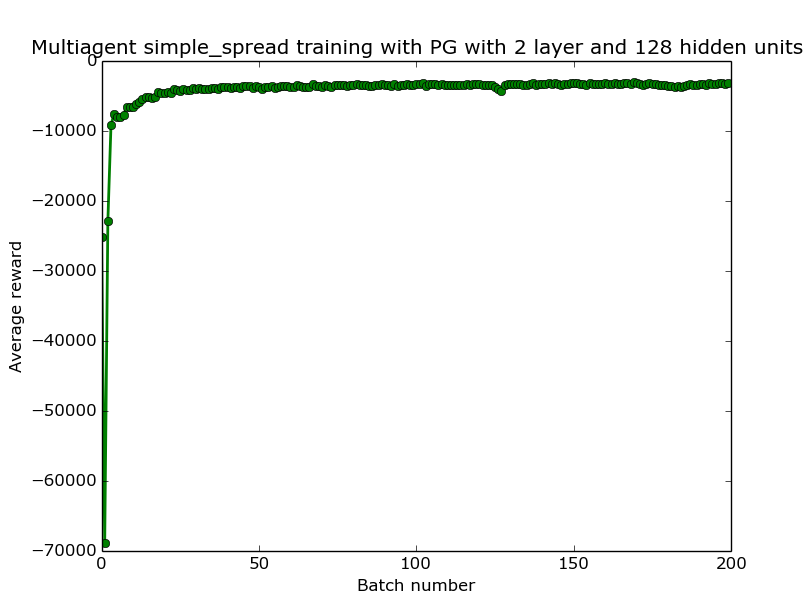
\includegraphics[scale=0.25]{pg_2_128_gamma1}
    \caption{Average reward over time when training PG with 2 layers and 128 hidden units.}
\label{fig:pg_2_128_gamma1}
\end{figure}

Figures ~\ref{fig:pg_1_16_gamma1}, ~\ref{fig:pg_1_32_gamma95}  and ~\ref{fig:pg_2_128_gamma1} show our initial results from training with different policy network sizes. We can see that although there is a significant improvement in average reward from the start of training, the average reward is still well below 0, indicating that the agents are not able to find an optimal strategy to cooperate and cover all of the target landmarks. This result is to be expected as policy gradient will be very unstable due to the non-stationary environment from the point of view of any given agent during training. When we increased the number of layers and units per layer we saw the network reach convergence quicker, but it was still not able to improve substantially, indicating that the algorithm itself could be a bottleneck on performance as opposed to the size of the policy networks.

\bibliography{milestone}
\bibliographystyle{icml2018}

\end{document}

